% Created by tikzDevice version 0.6.2-92-0ad2792 on 2013-01-11 06:36:49
% !TEX encoding = UTF-8 Unicode
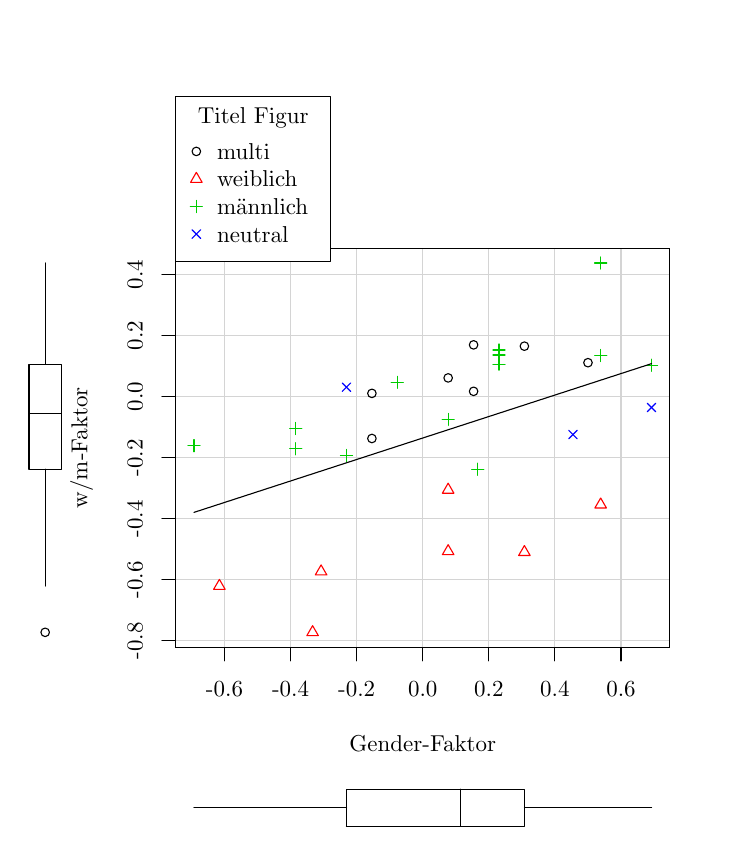
\begin{tikzpicture}[x=1pt,y=1pt]
\definecolor[named]{fillColor}{rgb}{1.00,1.00,1.00}
\path[use as bounding box,fill=fillColor,fill opacity=0.00] (0,0) rectangle (252.94,289.08);
\begin{scope}
\path[clip] (  0.00, 65.25) rectangle ( 12.65,209.40);
\definecolor[named]{drawColor}{rgb}{0.00,0.00,0.00}

\path[draw=drawColor,line width= 0.4pt,line join=round,line cap=round] (  0.47,129.51) --
	( 12.18,129.51) --
	( 12.18,167.50) --
	(  0.47,167.50) --
	(  0.47,129.51);

\path[draw=drawColor,line width= 0.4pt,line join=round,line cap=round] (  0.47,149.68) --
	( 12.18,149.68);

\path[draw=drawColor,line width= 0.4pt,line join=round,line cap=round] (  6.32, 87.32) --
	(  6.32,129.51);

\path[draw=drawColor,line width= 0.4pt,line join=round,line cap=round] (  6.32,167.50) --
	(  6.32,204.06);

\path[draw=drawColor,line width= 0.4pt,line join=round,line cap=round] (  6.32, 70.59) circle (  1.55);
\end{scope}
\begin{scope}
\path[clip] ( 53.48,  0.00) rectangle (232.03, 14.45);
\definecolor[named]{drawColor}{rgb}{0.00,0.00,0.00}

\path[draw=drawColor,line width= 0.4pt,line join=round,line cap=round] (115.20,  0.54) --
	(115.20, 13.92) --
	(179.49, 13.92) --
	(179.49,  0.54) --
	(115.20,  0.54);

\path[draw=drawColor,line width= 0.4pt,line join=round,line cap=round] (156.53,  0.54) --
	(156.53, 13.92);

\path[draw=drawColor,line width= 0.4pt,line join=round,line cap=round] ( 60.10,  7.23) --
	(115.20,  7.23);

\path[draw=drawColor,line width= 0.4pt,line join=round,line cap=round] (179.49,  7.23) --
	(225.42,  7.23);
\end{scope}
\begin{scope}
\path[clip] (  0.00,  0.00) rectangle (252.94,289.08);
\definecolor[named]{drawColor}{rgb}{0.00,0.00,0.00}

\path[draw=drawColor,line width= 0.4pt,line join=round,line cap=round] ( 71.12, 65.25) -- (214.39, 65.25);

\path[draw=drawColor,line width= 0.4pt,line join=round,line cap=round] ( 71.12, 65.25) -- ( 71.12, 60.27);

\path[draw=drawColor,line width= 0.4pt,line join=round,line cap=round] ( 95.00, 65.25) -- ( 95.00, 60.27);

\path[draw=drawColor,line width= 0.4pt,line join=round,line cap=round] (118.88, 65.25) -- (118.88, 60.27);

\path[draw=drawColor,line width= 0.4pt,line join=round,line cap=round] (142.76, 65.25) -- (142.76, 60.27);

\path[draw=drawColor,line width= 0.4pt,line join=round,line cap=round] (166.64, 65.25) -- (166.64, 60.27);

\path[draw=drawColor,line width= 0.4pt,line join=round,line cap=round] (190.52, 65.25) -- (190.52, 60.27);

\path[draw=drawColor,line width= 0.4pt,line join=round,line cap=round] (214.39, 65.25) -- (214.39, 60.27);

\node[text=drawColor,anchor=base,inner sep=0pt, outer sep=0pt, scale=  0.83] at ( 71.12, 47.32) {-0.6};

\node[text=drawColor,anchor=base,inner sep=0pt, outer sep=0pt, scale=  0.83] at ( 95.00, 47.32) {-0.4};

\node[text=drawColor,anchor=base,inner sep=0pt, outer sep=0pt, scale=  0.83] at (118.88, 47.32) {-0.2};

\node[text=drawColor,anchor=base,inner sep=0pt, outer sep=0pt, scale=  0.83] at (142.76, 47.32) {0.0};

\node[text=drawColor,anchor=base,inner sep=0pt, outer sep=0pt, scale=  0.83] at (166.64, 47.32) {0.2};

\node[text=drawColor,anchor=base,inner sep=0pt, outer sep=0pt, scale=  0.83] at (190.52, 47.32) {0.4};

\node[text=drawColor,anchor=base,inner sep=0pt, outer sep=0pt, scale=  0.83] at (214.39, 47.32) {0.6};

\path[draw=drawColor,line width= 0.4pt,line join=round,line cap=round] ( 53.48, 67.54) -- ( 53.48,199.88);

\path[draw=drawColor,line width= 0.4pt,line join=round,line cap=round] ( 53.48, 67.54) -- ( 48.50, 67.54);

\path[draw=drawColor,line width= 0.4pt,line join=round,line cap=round] ( 53.48, 89.60) -- ( 48.50, 89.60);

\path[draw=drawColor,line width= 0.4pt,line join=round,line cap=round] ( 53.48,111.65) -- ( 48.50,111.65);

\path[draw=drawColor,line width= 0.4pt,line join=round,line cap=round] ( 53.48,133.71) -- ( 48.50,133.71);

\path[draw=drawColor,line width= 0.4pt,line join=round,line cap=round] ( 53.48,155.77) -- ( 48.50,155.77);

\path[draw=drawColor,line width= 0.4pt,line join=round,line cap=round] ( 53.48,177.82) -- ( 48.50,177.82);

\path[draw=drawColor,line width= 0.4pt,line join=round,line cap=round] ( 53.48,199.88) -- ( 48.50,199.88);

\node[text=drawColor,rotate= 90.00,anchor=base,inner sep=0pt, outer sep=0pt, scale=  0.83] at ( 41.53, 67.54) {-0.8};

\node[text=drawColor,rotate= 90.00,anchor=base,inner sep=0pt, outer sep=0pt, scale=  0.83] at ( 41.53, 89.60) {-0.6};

\node[text=drawColor,rotate= 90.00,anchor=base,inner sep=0pt, outer sep=0pt, scale=  0.83] at ( 41.53,111.65) {-0.4};

\node[text=drawColor,rotate= 90.00,anchor=base,inner sep=0pt, outer sep=0pt, scale=  0.83] at ( 41.53,133.71) {-0.2};

\node[text=drawColor,rotate= 90.00,anchor=base,inner sep=0pt, outer sep=0pt, scale=  0.83] at ( 41.53,155.77) {0.0};

\node[text=drawColor,rotate= 90.00,anchor=base,inner sep=0pt, outer sep=0pt, scale=  0.83] at ( 41.53,177.82) {0.2};

\node[text=drawColor,rotate= 90.00,anchor=base,inner sep=0pt, outer sep=0pt, scale=  0.83] at ( 41.53,199.88) {0.4};

\path[draw=drawColor,line width= 0.4pt,line join=round,line cap=round] ( 53.48, 65.25) --
	(232.03, 65.25) --
	(232.03,209.40) --
	( 53.48,209.40) --
	( 53.48, 65.25);
\end{scope}
\begin{scope}
\path[clip] ( 12.65, 14.45) rectangle (252.94,289.08);
\definecolor[named]{drawColor}{rgb}{0.00,0.00,0.00}

\node[text=drawColor,anchor=base,inner sep=0pt, outer sep=0pt, scale=  0.83] at (142.76, 27.40) {Gender-Faktor};

\node[text=drawColor,rotate= 90.00,anchor=base,inner sep=0pt, outer sep=0pt, scale=  0.83] at ( 21.61,137.33) {w/m-Faktor};
\end{scope}
\begin{scope}
\path[clip] ( 53.48, 65.25) rectangle (232.03,209.40);
\definecolor[named]{drawColor}{rgb}{0.83,0.83,0.83}

\path[draw=drawColor,line width= 0.4pt,line join=round,line cap=round] ( 71.12, 65.25) -- ( 71.12,209.40);

\path[draw=drawColor,line width= 0.4pt,line join=round,line cap=round] ( 95.00, 65.25) -- ( 95.00,209.40);

\path[draw=drawColor,line width= 0.4pt,line join=round,line cap=round] (118.88, 65.25) -- (118.88,209.40);

\path[draw=drawColor,line width= 0.4pt,line join=round,line cap=round] (142.76, 65.25) -- (142.76,209.40);

\path[draw=drawColor,line width= 0.4pt,line join=round,line cap=round] (166.64, 65.25) -- (166.64,209.40);

\path[draw=drawColor,line width= 0.4pt,line join=round,line cap=round] (190.52, 65.25) -- (190.52,209.40);

\path[draw=drawColor,line width= 0.4pt,line join=round,line cap=round] (214.39, 65.25) -- (214.39,209.40);

\path[draw=drawColor,line width= 0.4pt,line join=round,line cap=round] ( 53.48, 67.54) -- (232.03, 67.54);

\path[draw=drawColor,line width= 0.4pt,line join=round,line cap=round] ( 53.48, 89.60) -- (232.03, 89.60);

\path[draw=drawColor,line width= 0.4pt,line join=round,line cap=round] ( 53.48,111.65) -- (232.03,111.65);

\path[draw=drawColor,line width= 0.4pt,line join=round,line cap=round] ( 53.48,133.71) -- (232.03,133.71);

\path[draw=drawColor,line width= 0.4pt,line join=round,line cap=round] ( 53.48,155.77) -- (232.03,155.77);

\path[draw=drawColor,line width= 0.4pt,line join=round,line cap=round] ( 53.48,177.82) -- (232.03,177.82);

\path[draw=drawColor,line width= 0.4pt,line join=round,line cap=round] ( 53.48,199.88) -- (232.03,199.88);
\end{scope}
\begin{scope}
\path[clip] (  0.00,  0.00) rectangle (252.94,289.08);
\definecolor[named]{drawColor}{rgb}{0.00,0.00,0.00}

\path[draw=drawColor,line width= 0.4pt,line join=round,line cap=round] ( 53.48, 65.25) --
	(232.03, 65.25) --
	(232.03,209.40) --
	( 53.48,209.40) --
	( 53.48, 65.25);
\end{scope}
\begin{scope}
\path[clip] ( 53.48, 65.25) rectangle (232.03,209.40);
\definecolor[named]{drawColor}{rgb}{0.00,0.00,0.00}

\path[draw=drawColor,line width= 0.4pt,line join=round,line cap=round] (151.94,162.52) circle (  1.55);

\path[draw=drawColor,line width= 0.4pt,line join=round,line cap=round] (124.39,140.63) circle (  1.55);

\path[draw=drawColor,line width= 0.4pt,line join=round,line cap=round] (124.39,156.93) circle (  1.55);

\path[draw=drawColor,line width= 0.4pt,line join=round,line cap=round] (161.13,157.67) circle (  1.55);

\path[draw=drawColor,line width= 0.4pt,line join=round,line cap=round] (161.13,174.46) circle (  1.55);

\path[draw=drawColor,line width= 0.4pt,line join=round,line cap=round] (179.49,173.99) circle (  1.55);

\path[draw=drawColor,line width= 0.4pt,line join=round,line cap=round] (202.46,168.02) circle (  1.55);
\definecolor[named]{drawColor}{rgb}{1.00,0.00,0.00}

\path[draw=drawColor,line width= 0.4pt,line join=round,line cap=round] (102.96, 73.00) --
	(105.04, 69.38) --
	(100.87, 69.38) --
	(102.96, 73.00);

\path[draw=drawColor,line width= 0.4pt,line join=round,line cap=round] (151.94,102.27) --
	(154.03, 98.65) --
	(149.85, 98.65) --
	(151.94,102.27);

\path[draw=drawColor,line width= 0.4pt,line join=round,line cap=round] ( 69.28, 89.73) --
	( 71.37, 86.11) --
	( 67.19, 86.11) --
	( 69.28, 89.73);

\path[draw=drawColor,line width= 0.4pt,line join=round,line cap=round] (151.94,124.48) --
	(154.03,120.86) --
	(149.85,120.86) --
	(151.94,124.48);

\path[draw=drawColor,line width= 0.4pt,line join=round,line cap=round] (106.02, 94.95) --
	(108.11, 91.33) --
	(103.93, 91.33) --
	(106.02, 94.95);

\path[draw=drawColor,line width= 0.4pt,line join=round,line cap=round] (179.49,101.95) --
	(181.58, 98.34) --
	(177.41, 98.34) --
	(179.49,101.95);

\path[draw=drawColor,line width= 0.4pt,line join=round,line cap=round] (207.05,119.13) --
	(209.13,115.52) --
	(204.96,115.52) --
	(207.05,119.13);
\definecolor[named]{drawColor}{rgb}{0.00,0.80,0.00}

\path[draw=drawColor,line width= 0.4pt,line join=round,line cap=round] (160.46,129.51) -- (164.85,129.51);

\path[draw=drawColor,line width= 0.4pt,line join=round,line cap=round] (162.66,127.32) -- (162.66,131.70);

\path[draw=drawColor,line width= 0.4pt,line join=round,line cap=round] (113.01,134.48) -- (117.39,134.48);

\path[draw=drawColor,line width= 0.4pt,line join=round,line cap=round] (115.20,132.29) -- (115.20,136.68);

\path[draw=drawColor,line width= 0.4pt,line join=round,line cap=round] (149.75,147.54) -- (154.13,147.54);

\path[draw=drawColor,line width= 0.4pt,line join=round,line cap=round] (151.94,145.34) -- (151.94,149.73);

\path[draw=drawColor,line width= 0.4pt,line join=round,line cap=round] (131.38,160.91) -- (135.76,160.91);

\path[draw=drawColor,line width= 0.4pt,line join=round,line cap=round] (133.57,158.72) -- (133.57,163.10);

\path[draw=drawColor,line width= 0.4pt,line join=round,line cap=round] (168.12,167.50) -- (172.50,167.50);

\path[draw=drawColor,line width= 0.4pt,line join=round,line cap=round] (170.31,165.31) -- (170.31,169.69);

\path[draw=drawColor,line width= 0.4pt,line join=round,line cap=round] ( 94.64,136.94) -- ( 99.03,136.94);

\path[draw=drawColor,line width= 0.4pt,line join=round,line cap=round] ( 96.83,134.75) -- ( 96.83,139.13);

\path[draw=drawColor,line width= 0.4pt,line join=round,line cap=round] (223.22,167.06) -- (227.61,167.06);

\path[draw=drawColor,line width= 0.4pt,line join=round,line cap=round] (225.42,164.87) -- (225.42,169.26);

\path[draw=drawColor,line width= 0.4pt,line join=round,line cap=round] ( 94.64,144.27) -- ( 99.03,144.27);

\path[draw=drawColor,line width= 0.4pt,line join=round,line cap=round] ( 96.83,142.07) -- ( 96.83,146.46);

\path[draw=drawColor,line width= 0.4pt,line join=round,line cap=round] (204.86,204.06) -- (209.24,204.06);

\path[draw=drawColor,line width= 0.4pt,line join=round,line cap=round] (207.05,201.87) -- (207.05,206.25);

\path[draw=drawColor,line width= 0.4pt,line join=round,line cap=round] ( 57.90,138.03) -- ( 62.29,138.03);

\path[draw=drawColor,line width= 0.4pt,line join=round,line cap=round] ( 60.10,135.84) -- ( 60.10,140.22);

\path[draw=drawColor,line width= 0.4pt,line join=round,line cap=round] (168.12,170.81) -- (172.50,170.81);

\path[draw=drawColor,line width= 0.4pt,line join=round,line cap=round] (170.31,168.61) -- (170.31,173.00);

\path[draw=drawColor,line width= 0.4pt,line join=round,line cap=round] (204.86,170.64) -- (209.24,170.64);

\path[draw=drawColor,line width= 0.4pt,line join=round,line cap=round] (207.05,168.45) -- (207.05,172.83);

\path[draw=drawColor,line width= 0.4pt,line join=round,line cap=round] (168.12,172.61) -- (172.50,172.61);

\path[draw=drawColor,line width= 0.4pt,line join=round,line cap=round] (170.31,170.42) -- (170.31,174.80);
\definecolor[named]{drawColor}{rgb}{0.00,0.00,1.00}

\path[draw=drawColor,line width= 0.4pt,line join=round,line cap=round] (223.87,150.28) -- (226.97,153.38);

\path[draw=drawColor,line width= 0.4pt,line join=round,line cap=round] (223.87,153.38) -- (226.97,150.28);

\path[draw=drawColor,line width= 0.4pt,line join=round,line cap=round] (195.48,140.50) -- (198.58,143.60);

\path[draw=drawColor,line width= 0.4pt,line join=round,line cap=round] (195.48,143.60) -- (198.58,140.50);

\path[draw=drawColor,line width= 0.4pt,line join=round,line cap=round] (113.65,157.61) -- (116.75,160.71);

\path[draw=drawColor,line width= 0.4pt,line join=round,line cap=round] (113.65,160.71) -- (116.75,157.61);
\definecolor[named]{drawColor}{rgb}{0.00,0.00,0.00}

\path[draw=drawColor,line width= 0.4pt,line join=round,line cap=round] ( 60.10,113.93) --
	(225.42,167.67);
\end{scope}
\begin{scope}
\path[clip] ( 12.65, 14.45) rectangle (252.94,289.08);
\definecolor[named]{drawColor}{rgb}{0.00,0.00,0.00}
\definecolor[named]{fillColor}{rgb}{1.00,1.00,1.00}

\path[draw=drawColor,line width= 0.4pt,line join=round,line cap=round,fill=fillColor] ( 53.48,264.28) rectangle (109.50,204.52);

\path[draw=drawColor,line width= 0.4pt,line join=round,line cap=round] ( 60.95,244.36) circle (  1.55);
\definecolor[named]{drawColor}{rgb}{1.00,0.00,0.00}

\path[draw=drawColor,line width= 0.4pt,line join=round,line cap=round] ( 60.95,236.81) --
	( 63.04,233.19) --
	( 58.87,233.19) --
	( 60.95,236.81);
\definecolor[named]{drawColor}{rgb}{0.00,0.80,0.00}

\path[draw=drawColor,line width= 0.4pt,line join=round,line cap=round] ( 58.76,224.44) -- ( 63.15,224.44);

\path[draw=drawColor,line width= 0.4pt,line join=round,line cap=round] ( 60.95,222.25) -- ( 60.95,226.63);
\definecolor[named]{drawColor}{rgb}{0.00,0.00,1.00}

\path[draw=drawColor,line width= 0.4pt,line join=round,line cap=round] ( 59.40,212.93) -- ( 62.50,216.03);

\path[draw=drawColor,line width= 0.4pt,line join=round,line cap=round] ( 59.40,216.03) -- ( 62.50,212.93);
\definecolor[named]{drawColor}{rgb}{0.00,0.00,0.00}

\node[text=drawColor,anchor=base,inner sep=0pt, outer sep=0pt, scale=  0.83] at ( 81.49,254.32) {Titel Figur};

\node[text=drawColor,anchor=base west,inner sep=0pt, outer sep=0pt, scale=  0.83] at ( 68.42,241.50) {multi};

\node[text=drawColor,anchor=base west,inner sep=0pt, outer sep=0pt, scale=  0.83] at ( 68.42,231.54) {weiblich};

\node[text=drawColor,anchor=base west,inner sep=0pt, outer sep=0pt, scale=  0.83] at ( 68.42,221.58) {männlich};

\node[text=drawColor,anchor=base west,inner sep=0pt, outer sep=0pt, scale=  0.83] at ( 68.42,211.62) {neutral};
\end{scope}
\end{tikzpicture}
